\documentclass[11pt]{article}
\usepackage[utf8]{inputenc}
\usepackage[brazil]{babel}

\usepackage{float}
\usepackage{amsmath}
\usepackage{amssymb}
\usepackage{graphicx}
\newtheorem{theorem}{Teorema}[section]

\title{MO420 - TP de Planos de Cortes}
\author{RA009206 - Luís Guilherme Fernandes Pereira \\
RA044072 - Igor Ribeiro de Assis}
\date{Trabalho 3 - 1o semestre de 2009}

\begin{document}
\maketitle

\section{Introdução}

Neste trabalho prático, estudamos o problema de planos de cortes e
Branch and Cut, implementamos essa técnica no resolvedor XPress e
usamo-la para resolver o problema de \emph{minimum stabbing number}
(STAB).

\section{Formulação}

A seguinte formulação para o problema STAB foi utilizada.

\begin{align}
 min & \hspace{8pt}y\\
  s.a & \hspace{2pt}\sum_{e \in \delta (i)}{x_e} = 1 \label{grau} \\
      & \sum_{e \in E(S)}{x_e} \le (|S|-1)/2, \hspace{4pt} \forall S
  \subset P, \hspace{4pt} |S|
  \hspace{4pt} impar \label{exp} \\
      & \sum_{e \in I(r_{ij})}{x_e} \le y, \forall (i,j) \in N \times N,
    i < j \label{inter}
\end{align}

As restrições \eqref{grau} e \eqref{exp} são as restrições do problema
de emparelhamento perfeito (note que se a restrição de grau fosse do
tipo $\le$ teríamos a formulação emparelhamento máximo). As restrições
\eqref{grau} são restrições de grau e garantem que em cada vértice
exatamente uma aresta incidente nele tem o valor $x_e = 1$. As do tipo
\eqref{exp} embora não necessárias na formulação inteira do problema
do emparelhamento, ao se resolver o programa linear relaxado
correspondente elas evitam soluções com valores fracionários como na
figura \ref{fig:ciclo_impar}, e mais, são necessárias na descrição da
envoltória convexa [REFERÊNCIA DO ARTIGO AQUI].

Intuitivamente essas restrições dizem que para todo conjunto ímpar de
vértices, deve exister algum vértice ``casando'' com alguem de fora do
conjunto, observe que é importante que a $|S|$ seja ímpar caso
contrário estaríamos excluindo soluções válidas.

A variável $y$, utilizada no último grupo de restrições e na função
objetivo corresponde a um limite superior para o número de
intersecções de uma reta (das retas consideradas tendo em vista a
proposição $1$) com os segmentos do emparelhamento perfeito
encontrado, ou seja, a váriavel $y$ é um limite superior para o
$sn(M)$. Como o problema é de minimização da variável $y$, em qualquer
solução ótima no mínimo uma restrição do tipo \eqref{inter} será
satisfeita na igualdade.

\begin{figure}[H]
\centering
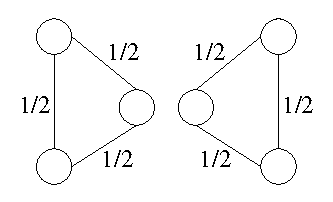
\includegraphics[scale=0.50]{ciclos}
\caption{Solução inválida do emparelhamento satisfazendo as restrições
  de grau}
\label{fig:ciclo_impar}
\end{figure}

Note que o número de restrições do tipo \eqref{exp} é exponencial,
portanto não é possível utilizar essa formulação com todas as
restrições é necessário um algoritmo de \emph{branch-and-cut}

Vejamos agora restrições alternativas para as do tipo \eqref{exp}, que
ao invés de somarem sobre as arestas do conjunto $S$, somam sobre as
arestas do corte cuja praia é $S$.

\begin{align}
  \sum_{e \in S}{x_e} \ge 1, \hspace{4pt}|S|\hspace{4pt} impar \label{corte}
\end{align}

Vamos mostrar que \eqref{corte} e \eqref{exp} são equivalentes.

Fixe um conjunto $S$ e seja $x^*$ uma solução do problema linear acima
que não satisfaz as restrições \eqref{exp}. Temos:

\begin{align}
  2\sum_{e \in E(S)}x_e^* > (|S| - 1)
\end{align}

Para o conjunto $S$,

\begin{align}
  \sum_{e \in \delta (S)}x_e^* = \sum_{i \in S}\sum_{e \in \delta
    (i)}x_e^* - 2\sum_{e \in E(S)}x_e^* < \sum_{i \in S}\sum_{e in
    \delta (i)}x_e^* - (|S| - 1)
\end{align}

Mas pelo fato de $x^*$ satisfazer as restrições de grau temos $\sum_{i
  \in S}\sum_{e \in \delta (i)}x_e^* = |S|$, portanto, $\sum_{e \in
  \delta (S)} < 1$, e $x^*$ não satisfaz \eqref{corte}. De maneira
análoga obtemos que se uma solução não satisfaz \eqref{corte} não
satisfaz \eqref{exp}.

Suponha agora que $x^*$ é uma solução válida para \eqref{exp}, então:

\begin{align}
  2\sum_{e \in E(S)}x_e^* \le (|S| - 1)
\end{align}

E,

\begin{align}
  \sum_{e \in \delta (S)}x_e^* = \sum_{i \in S}\sum_{e \in \delta
    (i)}x_e^* - 2\sum_{e \in E(S)}x_e^* \ge \sum_{i \in S}\sum_{e in
    \delta (i)}x_e^* - (|S| - 1)
\end{align}

Portanto, como $x^*$ satisfaz as restrições de grau, $\sum_{e \in
  \delta (S)} \ge 1$, como queríamos.

\section{Cortes Exatos}
Os cortes exatos foram implementados de forma a gerar restrições da
forma \eqref{corte}, isto é, o problema de separação resolvido era de
encontrar cortes mínimos ímpares. Para isto foi utilizada a árvore de
Gomory-Hu.

Seja $G=(V,E)$ um grafo não orientado e $c$ uma função de custo
positiva associada as arestas de $G$. Uma \emph{árvore de Gomory-Hu}
$T=(V,F)$ é uma árvore e uma função custo associada as arestas, em que
para cada aresta $e = uv$ de $T$, $\delta_G(U)$, com $U$ o conjunto de
vértices de uma das componentes de $T-e$, é um u-v-corte mínimo, e o
valor do corte é o custo da aresta $e$ em $T$. Além disso, dado dois
vértices quaisquer $u$ e $v$ de $G$ o valor do u-v-corte mínimo é o
custo da menor aresta no caminho de $u$ à $v$ em $T$.

Na figura \ref{fig:gomoryhu} (baseada em figura de \cite{bondymurty})
temos um grafo $G$ e a árvore de Gomory-Hu correspondente.

\begin{figure}[H]
\centering
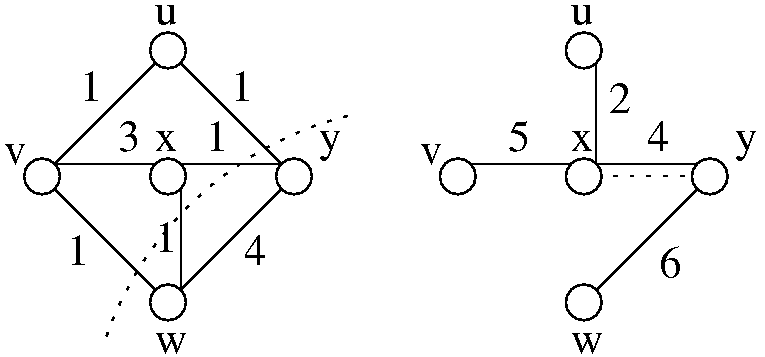
\includegraphics[scale=0.40]{gomoryhu}
\caption{Grafo e árvore de Gomory-Hu correspondente}
\label{fig:gomoryhu}
\end{figure}

No grafo temos marcado o corte separando os vértices $w$ e $v$ e na
árvore, a aresta correspondente ao corte.

\section{Heurísticas}

Implementamos duas estratégias heurísticas, sendo uma para separação de
cortes e outra para encontrar limitantes primais. 

\subsection{Heurística de Separação de Cortes}

Baseado na restrição \eqref{exp}, podemos encontrar desigualdades
violadas de maneira simples, e executamos o seguinte algoritmo: para
toda aresta $e$, ligando os vértices $i$ e $j$, de valor relaxado \( 0,5
< x_e < 1 \), verificamos se existem vértices $k$ tais que \( x_{ij} +
x_{ik} + x_{jk} > 1 \). Caso encontremos esses ciclos, adicionamos a
seguinte desigualdade válida para cada um deles: 

\begin{equation}
 x_{ij} + x_{ik} + x_{jk} \leq 1
\end{equation}

Como é simples constatar, essa desigualdade corresponde à restrição
\eqref{exp} para um conjunto $S$ de tamanho $3$. 

Para cada aresta, fazemos uma busca nos vértices. Logo, a complexidade
da separação heurística é $O(|V||E|)$

\subsection{Heurística Primal}

Bons limitantes primais, como será mostrado na seção de resultados,
ajudam sobremaneira na resolução de problemas difíceis, principalmente
quando se usam estratégias de \emph{branching}.

Dada uma solução da relaxação linear $x^*$, podemos encontrar um
emparelhamento perfeito da seguinte forma (e, portanto, uma solução
viável para o STAB): para cada aresta $x^*_e$, arrendondamos o seu valor
para $0$ ou $1$, de forma que a restrição \eqref{grau} seja satisfeita
para todo vértice. 

Inicialmente testamos o seguinte algoritmo: para cada vértice $i$ não
emparelhado, encontre o vértice $j$ não emparelhado cuja aresta $x_ij$
tem o maior valor relaxado. Marque $i$ e $j$ como emparelhados, e
arredonde $x_ij$ para 1. $\forall k \notin {i,j}$, $x_ik$ e $x_jk$ são
marcados como zero. Essa heurística primal raramente melhorava a
solução e não contribuiu para a redução do número de nós pesquisados
pelos algoritmos de \emph{branching}. Essa heurística tem complexidade
$O(|V||E|)$ 

Implementamos um algoritmo muito semelhante, mas que diferia na ordem de
busca das arestas a serem arredondadas para valores integrais, e
obtivemos resultados incrivelmente superiores. Inicialmente, ordenamos
as arestas decrescentemente por valor relaxado. Percorrendo-as nessa
ordem, caso elas ligassem dois vértices $i$ e $j$ ainda não emparelhados,
arredondava-se seu valor para $1$, $i$ e $j$ eram marcados como
emparelhados. Caso contrário, seu valor era marcado como $0$. 

Nesse algoritmo ordenamos as arestas e depois percorremo-nas executando
operações triviais. A ordenação domina a computação dessa heurística e,
portanto, sua complexidade é dada por $O(|E| log (|E|))$.


\section{Tempos}

Na tabela \ref{tab:tempos} há os tempos envolvidos para cada execução,
medidos como soma de tempo de usuário e tempo de sistema no programa
\texttt{time}. A linha de cabeçalho corresponde à forma de entrada do
programa, isto é, \textbf{b} indica \emph{branch and bound} puro,
\textbf{r} indica o algoritmo planos de corte, e \textbf{f} indica o
algoritmo de \emph{branch and cut}, executado com profundidade máxima
para cortes de $2$. Os dois dígitos indicam se houve uso
de heurísticas, $1$ indica que houve, e $0$ o contrário. O primeiro
dígito indica o uso da heurística primal,  e o segundo dígito da
heurística de geração de cortes. Em negrito, os valores em que não foi
possível encontrar solução inteira (não coincidentemente, justamente os
casos de algoritmo de plano de cortes puro sem heurística primal).



\begin{table}[htb]
\begin{tiny}
\centering
\begin{tabular}[b]{|c|c|c|c|c|c|c|c|c|c|c|}
\hline
& b00 & b10 & r00 & r01 & r10 & r11 & f00 & f01 & f10 & f11 \\ \hline
eil76\_66 & 25.03 & 26.16 & \textbf{38.16} & \textbf{34.4} & 38.9 & 35.23 & 111.81 & 93.42 & 67.11 & 95.94 \\ \hline
kroC100\_70 & 28.55 & 23.4 & \textbf{26.42} & \textbf{29.78} & 26.77 & 29.74 & 94.62 & 108.71 & 80.17 & 107.47 \\ \hline
kroB100\_60 & 37.73 & 13.03 & \textbf{22.88} & \textbf{18.58} & 23.23 & 18.7 & 185.72 & 91.59 & 370.71 & 104.05 \\ \hline
brd14051\_60 & 34.91 & 11.61 & \textbf{15.29} & \textbf{20.06} & 15.55 & 20.45 & 65.48 & 60.95 & 42.4 & 50.96 \\ \hline
gil262\_70 & 72.24 & 23.33 & \textbf{108.17} & \textbf{62.44} & 111.8 & 63.32 & 119.76 & 168.53 & 89.96 & 125.07 \\ \hline
kroB100\_70 & 84.21 & 110.06 & \textbf{34.99} & \textbf{31.12} & 35.63 & 31.46 & 301.14 & 276.51 & 177.77 & 204.11 \\ \hline
eil51\_50 & 11.58 & 4.94 & \textbf{7.21} & \textbf{10.22} & 6.9 & 10.4 & 34.25 & 22.48 & 15.64 & 15.0 \\ \hline
lin105\_60 & 8.64 & 10.77 & \textbf{9.43} & \textbf{9.09} & 9.5 & 9.2 & 63.39 & 82.48 & 37.16 & 16.38 \\ \hline
gil262\_60 & 16.12 & 7.62 & \textbf{22.55} & \textbf{25.17} & 22.81 & 25.55 & 53.84 & 82.39 & 18.33 & 13.6 \\ \hline
kroA100\_50 & 11.93 & 3.68 & \textbf{6.0} & \textbf{5.67} & 4.6 & 5.7 & 22.55 & 26.89 & 4.6 & 9.01 \\ \hline
brd14051\_70 & 23.5 & 24.57 & \textbf{81.98} & \textbf{29.41} & 83.44 & 29.73 & 124.66 & 87.04 & 88.74 & 90.42 \\ \hline
bier127\_60 & 15.53 & 6.51 & \textbf{54.56} & \textbf{47.17} & 17.14 & 22.51 & 75.25 & 62.3 & 11.86 & 11.63 \\ \hline
\end{tabular}
\end{tiny}
\caption{Tempos de execução para as instâncias sugeridas}
\label{tab:tempos}
\end{table}

Além da impossibilidade do algoritmo de planos de corte puro conseguir
encontrar uma solução viável sem o uso de heurística primal, podemos
observar que:

\begin{enumerate}
 \item Na maioria dos casos, o uso da heurística primal reduz
       sensivelmente o tempo de execução. Um contra exemplo é o
       algoritmo de \emph{branch and cut} para a instância
       kroB100\_60. O contrário pode ser observado em quase todos os
       outros casos, com destaque para a instância bier127\_60, que teve
       o tempo reduzido em um sexto. 
 \item O uso da heurística para encontrar planos de cortes não dá
       melhoras consistentes no tempo de exceção, com algumas honrosas
       exceções, como no plano de cortes puro para o brd14051\_70 e no
       \emph{branch and cut} para o kroB100\_60.
 \item Infelizmente, os melhores tempos de execução são quase sempre
       obtidos com o algoritmo de \emph{branch and bound} puro. O uso da
       heurística primal em geral melhora ainda mais esse tempo. O uso
       de estruturas de dados adequadas e uma implementação mais enxuta
       do XPRESS em comparação com o código de laboratório pode explicar
       em parte esse dado. Outra possibilidade é uma implementação
       imperfeita dos algoritmos. Ainda elencamos o fato de nossa
       heurística de separação não ser tão eficiente, e o algoritmo
       exato ter uma complexidade ruim, ainda que polinomial, o que
       contribui para delongar as execuções que realizam separação por
       cortes. 
\end{enumerate} 

\bibliographystyle{alpha}
\bibliography{ra009206-044072-texto.bib}

\end{document}
